\section{Versuchsaufbau}
Um in diesem Versuch das Trägheitsmoment eines Körpers zu berechnen, wird dieser auf einer drehbaren Achse 
befestigt, welche sich in einem Rahmen befindet. Diese Drillachse ist über eine Spiralfeder mit dem Rahmen verbunden,
sodass die Körper ausgelenkt werden können. Um zu vermeiden, dass sich die Spiralfeder verformt, werden die Körper
in der Versuchsdurchführung maximal um einen Winkel von 360° ausgelenkt. 

\begin{figure}
\centering
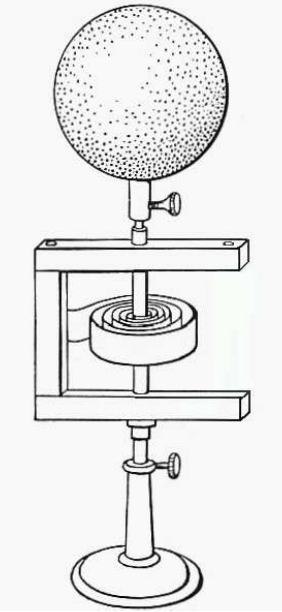
\includegraphics[scale=.5]{V101Bild.png}
\label{fig:abb2}
\caption{Der Versuchsaufbau.\cite[3]{anleitung101}}
\end{figure}